% Options for packages loaded elsewhere
\PassOptionsToPackage{unicode}{hyperref}
\PassOptionsToPackage{hyphens}{url}
\PassOptionsToPackage{dvipsnames,svgnames,x11names}{xcolor}
%
\documentclass[
  letterpaper,
  DIV=11,
  numbers=noendperiod]{scrreprt}

\usepackage{amsmath,amssymb}
\usepackage{lmodern}
\usepackage{iftex}
\ifPDFTeX
  \usepackage[T1]{fontenc}
  \usepackage[utf8]{inputenc}
  \usepackage{textcomp} % provide euro and other symbols
\else % if luatex or xetex
  \usepackage{unicode-math}
  \defaultfontfeatures{Scale=MatchLowercase}
  \defaultfontfeatures[\rmfamily]{Ligatures=TeX,Scale=1}
\fi
% Use upquote if available, for straight quotes in verbatim environments
\IfFileExists{upquote.sty}{\usepackage{upquote}}{}
\IfFileExists{microtype.sty}{% use microtype if available
  \usepackage[]{microtype}
  \UseMicrotypeSet[protrusion]{basicmath} % disable protrusion for tt fonts
}{}
\makeatletter
\@ifundefined{KOMAClassName}{% if non-KOMA class
  \IfFileExists{parskip.sty}{%
    \usepackage{parskip}
  }{% else
    \setlength{\parindent}{0pt}
    \setlength{\parskip}{6pt plus 2pt minus 1pt}}
}{% if KOMA class
  \KOMAoptions{parskip=half}}
\makeatother
\usepackage{xcolor}
\setlength{\emergencystretch}{3em} % prevent overfull lines
\setcounter{secnumdepth}{5}
% Make \paragraph and \subparagraph free-standing
\ifx\paragraph\undefined\else
  \let\oldparagraph\paragraph
  \renewcommand{\paragraph}[1]{\oldparagraph{#1}\mbox{}}
\fi
\ifx\subparagraph\undefined\else
  \let\oldsubparagraph\subparagraph
  \renewcommand{\subparagraph}[1]{\oldsubparagraph{#1}\mbox{}}
\fi

\usepackage{color}
\usepackage{fancyvrb}
\newcommand{\VerbBar}{|}
\newcommand{\VERB}{\Verb[commandchars=\\\{\}]}
\DefineVerbatimEnvironment{Highlighting}{Verbatim}{commandchars=\\\{\}}
% Add ',fontsize=\small' for more characters per line
\usepackage{framed}
\definecolor{shadecolor}{RGB}{241,243,245}
\newenvironment{Shaded}{\begin{snugshade}}{\end{snugshade}}
\newcommand{\AlertTok}[1]{\textcolor[rgb]{0.68,0.00,0.00}{#1}}
\newcommand{\AnnotationTok}[1]{\textcolor[rgb]{0.37,0.37,0.37}{#1}}
\newcommand{\AttributeTok}[1]{\textcolor[rgb]{0.40,0.45,0.13}{#1}}
\newcommand{\BaseNTok}[1]{\textcolor[rgb]{0.68,0.00,0.00}{#1}}
\newcommand{\BuiltInTok}[1]{\textcolor[rgb]{0.00,0.23,0.31}{#1}}
\newcommand{\CharTok}[1]{\textcolor[rgb]{0.13,0.47,0.30}{#1}}
\newcommand{\CommentTok}[1]{\textcolor[rgb]{0.37,0.37,0.37}{#1}}
\newcommand{\CommentVarTok}[1]{\textcolor[rgb]{0.37,0.37,0.37}{\textit{#1}}}
\newcommand{\ConstantTok}[1]{\textcolor[rgb]{0.56,0.35,0.01}{#1}}
\newcommand{\ControlFlowTok}[1]{\textcolor[rgb]{0.00,0.23,0.31}{#1}}
\newcommand{\DataTypeTok}[1]{\textcolor[rgb]{0.68,0.00,0.00}{#1}}
\newcommand{\DecValTok}[1]{\textcolor[rgb]{0.68,0.00,0.00}{#1}}
\newcommand{\DocumentationTok}[1]{\textcolor[rgb]{0.37,0.37,0.37}{\textit{#1}}}
\newcommand{\ErrorTok}[1]{\textcolor[rgb]{0.68,0.00,0.00}{#1}}
\newcommand{\ExtensionTok}[1]{\textcolor[rgb]{0.00,0.23,0.31}{#1}}
\newcommand{\FloatTok}[1]{\textcolor[rgb]{0.68,0.00,0.00}{#1}}
\newcommand{\FunctionTok}[1]{\textcolor[rgb]{0.28,0.35,0.67}{#1}}
\newcommand{\ImportTok}[1]{\textcolor[rgb]{0.00,0.46,0.62}{#1}}
\newcommand{\InformationTok}[1]{\textcolor[rgb]{0.37,0.37,0.37}{#1}}
\newcommand{\KeywordTok}[1]{\textcolor[rgb]{0.00,0.23,0.31}{#1}}
\newcommand{\NormalTok}[1]{\textcolor[rgb]{0.00,0.23,0.31}{#1}}
\newcommand{\OperatorTok}[1]{\textcolor[rgb]{0.37,0.37,0.37}{#1}}
\newcommand{\OtherTok}[1]{\textcolor[rgb]{0.00,0.23,0.31}{#1}}
\newcommand{\PreprocessorTok}[1]{\textcolor[rgb]{0.68,0.00,0.00}{#1}}
\newcommand{\RegionMarkerTok}[1]{\textcolor[rgb]{0.00,0.23,0.31}{#1}}
\newcommand{\SpecialCharTok}[1]{\textcolor[rgb]{0.37,0.37,0.37}{#1}}
\newcommand{\SpecialStringTok}[1]{\textcolor[rgb]{0.13,0.47,0.30}{#1}}
\newcommand{\StringTok}[1]{\textcolor[rgb]{0.13,0.47,0.30}{#1}}
\newcommand{\VariableTok}[1]{\textcolor[rgb]{0.07,0.07,0.07}{#1}}
\newcommand{\VerbatimStringTok}[1]{\textcolor[rgb]{0.13,0.47,0.30}{#1}}
\newcommand{\WarningTok}[1]{\textcolor[rgb]{0.37,0.37,0.37}{\textit{#1}}}

\providecommand{\tightlist}{%
  \setlength{\itemsep}{0pt}\setlength{\parskip}{0pt}}\usepackage{longtable,booktabs,array}
\usepackage{calc} % for calculating minipage widths
% Correct order of tables after \paragraph or \subparagraph
\usepackage{etoolbox}
\makeatletter
\patchcmd\longtable{\par}{\if@noskipsec\mbox{}\fi\par}{}{}
\makeatother
% Allow footnotes in longtable head/foot
\IfFileExists{footnotehyper.sty}{\usepackage{footnotehyper}}{\usepackage{footnote}}
\makesavenoteenv{longtable}
\usepackage{graphicx}
\makeatletter
\def\maxwidth{\ifdim\Gin@nat@width>\linewidth\linewidth\else\Gin@nat@width\fi}
\def\maxheight{\ifdim\Gin@nat@height>\textheight\textheight\else\Gin@nat@height\fi}
\makeatother
% Scale images if necessary, so that they will not overflow the page
% margins by default, and it is still possible to overwrite the defaults
% using explicit options in \includegraphics[width, height, ...]{}
\setkeys{Gin}{width=\maxwidth,height=\maxheight,keepaspectratio}
% Set default figure placement to htbp
\makeatletter
\def\fps@figure{htbp}
\makeatother

\KOMAoption{captions}{tableheading}
\makeatletter
\@ifpackageloaded{tcolorbox}{}{\usepackage[many]{tcolorbox}}
\@ifpackageloaded{fontawesome5}{}{\usepackage{fontawesome5}}
\definecolor{quarto-callout-color}{HTML}{909090}
\definecolor{quarto-callout-note-color}{HTML}{0758E5}
\definecolor{quarto-callout-important-color}{HTML}{CC1914}
\definecolor{quarto-callout-warning-color}{HTML}{EB9113}
\definecolor{quarto-callout-tip-color}{HTML}{00A047}
\definecolor{quarto-callout-caution-color}{HTML}{FC5300}
\definecolor{quarto-callout-color-frame}{HTML}{acacac}
\definecolor{quarto-callout-note-color-frame}{HTML}{4582ec}
\definecolor{quarto-callout-important-color-frame}{HTML}{d9534f}
\definecolor{quarto-callout-warning-color-frame}{HTML}{f0ad4e}
\definecolor{quarto-callout-tip-color-frame}{HTML}{02b875}
\definecolor{quarto-callout-caution-color-frame}{HTML}{fd7e14}
\makeatother
\makeatletter
\makeatother
\makeatletter
\@ifpackageloaded{bookmark}{}{\usepackage{bookmark}}
\makeatother
\makeatletter
\@ifpackageloaded{caption}{}{\usepackage{caption}}
\AtBeginDocument{%
\ifdefined\contentsname
  \renewcommand*\contentsname{Table of contents}
\else
  \newcommand\contentsname{Table of contents}
\fi
\ifdefined\listfigurename
  \renewcommand*\listfigurename{List of Figures}
\else
  \newcommand\listfigurename{List of Figures}
\fi
\ifdefined\listtablename
  \renewcommand*\listtablename{List of Tables}
\else
  \newcommand\listtablename{List of Tables}
\fi
\ifdefined\figurename
  \renewcommand*\figurename{Figure}
\else
  \newcommand\figurename{Figure}
\fi
\ifdefined\tablename
  \renewcommand*\tablename{Table}
\else
  \newcommand\tablename{Table}
\fi
}
\@ifpackageloaded{float}{}{\usepackage{float}}
\floatstyle{ruled}
\@ifundefined{c@chapter}{\newfloat{codelisting}{h}{lop}}{\newfloat{codelisting}{h}{lop}[chapter]}
\floatname{codelisting}{Listing}
\newcommand*\listoflistings{\listof{codelisting}{List of Listings}}
\makeatother
\makeatletter
\@ifpackageloaded{caption}{}{\usepackage{caption}}
\@ifpackageloaded{subcaption}{}{\usepackage{subcaption}}
\makeatother
\makeatletter
\@ifpackageloaded{tcolorbox}{}{\usepackage[many]{tcolorbox}}
\makeatother
\makeatletter
\@ifundefined{shadecolor}{\definecolor{shadecolor}{rgb}{.97, .97, .97}}
\makeatother
\makeatletter
\makeatother
\ifLuaTeX
  \usepackage{selnolig}  % disable illegal ligatures
\fi
\IfFileExists{bookmark.sty}{\usepackage{bookmark}}{\usepackage{hyperref}}
\IfFileExists{xurl.sty}{\usepackage{xurl}}{} % add URL line breaks if available
\urlstyle{same} % disable monospaced font for URLs
\hypersetup{
  pdftitle={Principles and Techniques of Data Science},
  pdfauthor={Kanu Grover; Bella Crouch},
  colorlinks=true,
  linkcolor={blue},
  filecolor={Maroon},
  citecolor={Blue},
  urlcolor={Blue},
  pdfcreator={LaTeX via pandoc}}

\title{Principles and Techniques of Data Science}
\usepackage{etoolbox}
\makeatletter
\providecommand{\subtitle}[1]{% add subtitle to \maketitle
  \apptocmd{\@title}{\par {\large #1 \par}}{}{}
}
\makeatother
\subtitle{Data 100}
\author{Kanu Grover \and Bella Crouch}
\date{}

\begin{document}
\maketitle
\ifdefined\Shaded\renewenvironment{Shaded}{\begin{tcolorbox}[frame hidden, enhanced, sharp corners, borderline west={3pt}{0pt}{shadecolor}, interior hidden, breakable, boxrule=0pt]}{\end{tcolorbox}}\fi

\renewcommand*\contentsname{Table of contents}
{
\hypersetup{linkcolor=}
\setcounter{tocdepth}{2}
\tableofcontents
}
\bookmarksetup{startatroot}

\hypertarget{welcome}{%
\chapter*{Welcome}\label{welcome}}
\addcontentsline{toc}{chapter}{Welcome}

\markboth{Welcome}{Welcome}

\hypertarget{about-the-course-notes}{%
\section*{About the Course Notes}\label{about-the-course-notes}}
\addcontentsline{toc}{section}{About the Course Notes}

\markright{About the Course Notes}

This text was developed for the Spring 2023 Edition of the UC Berkeley
course Data 100: Principles and Techniques of Data Science.

As this project in development during the Spring 2023 semester, these
course notes may be in flux. We appreciate your understanding. If you
spot any errors or would like to suggest any changes, please email us.
\textbf{Email}: data100.instructors@berkeley.edu

\bookmarksetup{startatroot}

\hypertarget{introduction}{%
\chapter{Introduction}\label{introduction}}

\begin{tcolorbox}[enhanced jigsaw, leftrule=.75mm, colframe=quarto-callout-note-color-frame, bottomrule=.15mm, colbacktitle=quarto-callout-note-color!10!white, opacitybacktitle=0.6, breakable, title=\textcolor{quarto-callout-note-color}{\faInfo}\hspace{0.5em}{Note}, opacityback=0, left=2mm, toprule=.15mm, bottomtitle=1mm, toptitle=1mm, rightrule=.15mm, colback=white, titlerule=0mm, coltitle=black, arc=.35mm]

\begin{itemize}
\tightlist
\item
  Understand the stages of the data science lifecycle.
\end{itemize}

\end{tcolorbox}

Data science is an interdisciplinary field with a variety of
applications. The field is rapidly evolving; many of the key technical
underpinnings in modern-day data science have been popularized during
the early 21\textsuperscript{st} century.

A true mastery of data science requires a deep theoretical understanding
and strong grasp of domain expertise. This course will help you build on
the former -- specifically, the foundation of your technical knowledge.
To do so, we've organized concepts in Data 100 around the \textbf{data
science lifecycle}: an iterative process that encompasses the various
statistical and computational building blocks of data science.

\hypertarget{data-science-lifecycle}{%
\section{Data Science Lifecycle}\label{data-science-lifecycle}}

The data science lifecycle is a high-level overview of the data science
workflow. It's a cycle of stages that a data scientist should explore as
they conduct a thorough analysis of a data-driven problem.

There are many variations of the key ideas present in the data science
lifecycle. In Data 100, we visualize the stages of the lifecycle using a
flow diagram. Notice how there are two entry points.

\hypertarget{ask-a-question}{%
\subsection{Ask a Question}\label{ask-a-question}}

Whether by curiosity or necessity, data scientists will constantly ask
questions. For example, in the business world, data scientists may be
interested in predicting the profit generated by a certain investment.
In the field of medicine, they may ask whether some patients are more
likely than others to benefit from a treatment.

Posing questions is one of the primary ways the data science lifecycle
begins. It helps to fully define the question. Here are some things you
should ask yourself before framing a question.

\begin{itemize}
\tightlist
\item
  What do we want to know?

  \begin{itemize}
  \tightlist
  \item
    A question that is too ambiguous may lead to confusion.
  \end{itemize}
\item
  What problems are we trying to solve?

  \begin{itemize}
  \tightlist
  \item
    The goal of asking a question should be clear in order to justify
    your efforts to stakeholders.
  \end{itemize}
\item
  What are the hypotheses we want to test?

  \begin{itemize}
  \tightlist
  \item
    This gives a clear perspective from which to analyze final results.
  \end{itemize}
\item
  What are the metrics for our success?

  \begin{itemize}
  \tightlist
  \item
    This gives a clear point to know when to finish the project.
  \end{itemize}
\end{itemize}

\hypertarget{obtain-data}{%
\subsection{Obtain Data}\label{obtain-data}}

The second entry point to the lifecycle is by obtaining data. A careful
analysis of any problem requires the use of data. Data may be readily
available to us, or we may have to embark on a process to collect it.
When doing so, its crucial to ask the following:

\begin{itemize}
\tightlist
\item
  What data do we have and what data do we need?

  \begin{itemize}
  \tightlist
  \item
    Define the units of the data (people, cities, points in time, etc.)
    and what features to measure.
  \end{itemize}
\item
  How will we sample more data?

  \begin{itemize}
  \tightlist
  \item
    Scrape the web, collect manually, etc.
  \end{itemize}
\item
  Is our data representative of the population we want to study?

  \begin{itemize}
  \tightlist
  \item
    If our data is not representative of our population of interest,
    then we can come to incorrect conclusions.
  \end{itemize}
\end{itemize}

Key procedures: \emph{data acquisition}, \emph{data cleaning}

\hypertarget{understand-the-data}{%
\subsection{Understand the Data}\label{understand-the-data}}

Raw data itself is not inherently useful. It's impossible to discern all
the patterns and relationships between variables without carefully
investigating them. Therefore, translating pure data to actionable
insights is a key job of a data scientist. For example, we may choose to
ask:

\begin{itemize}
\tightlist
\item
  How is our data organized and what does it contain?

  \begin{itemize}
  \tightlist
  \item
    Knowing what the data says about the world helps us better
    understand the world.
  \end{itemize}
\item
  Do we have relevant data?

  \begin{itemize}
  \tightlist
  \item
    If the data we have collected is not useful to the question at hand,
    then we must collected more data.
  \end{itemize}
\item
  What are the biases, anomalies, or other issues with the data?

  \begin{itemize}
  \tightlist
  \item
    These can lead to many false conclusions if ignored, so data
    scientists must always be aware of these issues.
  \end{itemize}
\item
  How do we transform the data to enable effective analysis?

  \begin{itemize}
  \tightlist
  \item
    Data is not always easy to interpret at first glance, so a data
    scientist should reveal these hidden insights.
  \end{itemize}
\end{itemize}

Key procedures: \emph{exploratory data analysis}, \emph{data
visualization}.

\hypertarget{understand-the-world}{%
\subsection{Understand the World}\label{understand-the-world}}

After observing the patterns in our data, we can begin answering our
question. This may require that we predict a quantity (machine
learning), or measure the effect of some treatment (inference).

From here, we may choose to report our results, or possibly conduct more
analysis. We may not be satisfied by our findings, or our initial
exploration may have brought up new questions that require a new data.

\begin{itemize}
\tightlist
\item
  What does the data say about the world?

  \begin{itemize}
  \tightlist
  \item
    Given our models, the data will lead us to certain conclusions about
    the real world.\\
  \end{itemize}
\item
  Does it answer our questions or accurately solve the problem?

  \begin{itemize}
  \tightlist
  \item
    If our model and data can not accomplish our goals, then we must
    reform our question, model, or both.\\
  \end{itemize}
\item
  How robust are our conclusions and can we trust the predictions?

  \begin{itemize}
  \tightlist
  \item
    Inaccurate models can lead to untrue conclusions.
  \end{itemize}
\end{itemize}

Key procedures: \emph{model creation}, \emph{prediction},
\emph{inference}.

\hypertarget{conclusion}{%
\section{Conclusion}\label{conclusion}}

The data science lifecycle is meant to be a set of general guidelines
rather than a hard list of requirements. In our journey exploring the
lifecycle, we'll cover both the underlying theory and technologies used
in data science, and we hope you'll build an appreciation for the field.

With that, let's begin by introducing one of the most important tools in
exploratory data analysis: \texttt{pandas}.

\bookmarksetup{startatroot}

\hypertarget{pandas-i}{%
\chapter{Pandas I}\label{pandas-i}}

\begin{tcolorbox}[enhanced jigsaw, leftrule=.75mm, colframe=quarto-callout-note-color-frame, bottomrule=.15mm, colbacktitle=quarto-callout-note-color!10!white, opacitybacktitle=0.6, breakable, title=\textcolor{quarto-callout-note-color}{\faInfo}\hspace{0.5em}{Note}, opacityback=0, left=2mm, toprule=.15mm, bottomtitle=1mm, toptitle=1mm, rightrule=.15mm, colback=white, titlerule=0mm, coltitle=black, arc=.35mm]

\begin{itemize}
\tightlist
\item
  Build familiarity with basic \texttt{pandas} syntax
\item
  Learn the methods of selecting and filtering data from a DataFrame.
\item
  Understand the differences between DataFrames and Series
\end{itemize}

\end{tcolorbox}

Data scientists work with data stored in a variety of formats. The
primary focus of this class is in understanding tabular data -- one of
the most widely used formats in data science. This note introduces
DataFrames, which are among the most popular representations of tabular
data. We'll also introduce \texttt{pandas}, the standard Python package
for manipulating data in DataFrames.

\hypertarget{introduction-to-exploratory-data-analysis}{%
\section{Introduction to Exploratory Data
Analysis}\label{introduction-to-exploratory-data-analysis}}

Imagine you collected, or have been given a box of data. What do you do
next?

The first step is to clean your data. \textbf{Data cleaning} often
corrects issues in the structure and formatting of data, including
missing values and unit conversions.

Data scientists have coined the term \textbf{exploratory data analysis
(EDA)} to describe the process of transforming raw data to insightful
observations. EDA is an \emph{open-ended} analysis of transforming,
visualizing, and summarizing patterns in data. In order to conduct EDA,
we first need to familiarize ourselves with \texttt{pandas} -- an
important programming tool.

\hypertarget{introduction-to-pandas}{%
\section{Introduction to Pandas}\label{introduction-to-pandas}}

\texttt{pandas} is a data analysis library to make data cleaning and
analysis fast and convenient in Python.

The \texttt{pandas} library adopts many coding idioms from
\texttt{NumPy}. The biggest difference is that \texttt{pandas} is
designed for working with tabular data, one of the most common data
formats (and the focus of Data 100).

Before writing any code, we must import \texttt{pandas} into our Python
environment.

\begin{Shaded}
\begin{Highlighting}[]
\CommentTok{\# \textasciigrave{}pd\textasciigrave{} is the conventional alias for Pandas, as \textasciigrave{}np\textasciigrave{} is for NumPy}
\ImportTok{import}\NormalTok{ pandas }\ImportTok{as}\NormalTok{ pd}
\end{Highlighting}
\end{Shaded}

\hypertarget{series-dataframes-and-indices}{%
\section{Series, DataFrames, and
Indices}\label{series-dataframes-and-indices}}

There are three fundamental data structures in \texttt{pandas}:

\begin{enumerate}
\def\labelenumi{\arabic{enumi}.}
\tightlist
\item
  \textbf{Series}: 1D labeled array data; best thought of as columnar
  data
\item
  \textbf{DataFrame}: 2D tabular data with rows and columns
\item
  \textbf{Index}: A sequence of row/column labels
\end{enumerate}

DataFrames, Series, and Indices can be represented visually in the
following diagram.

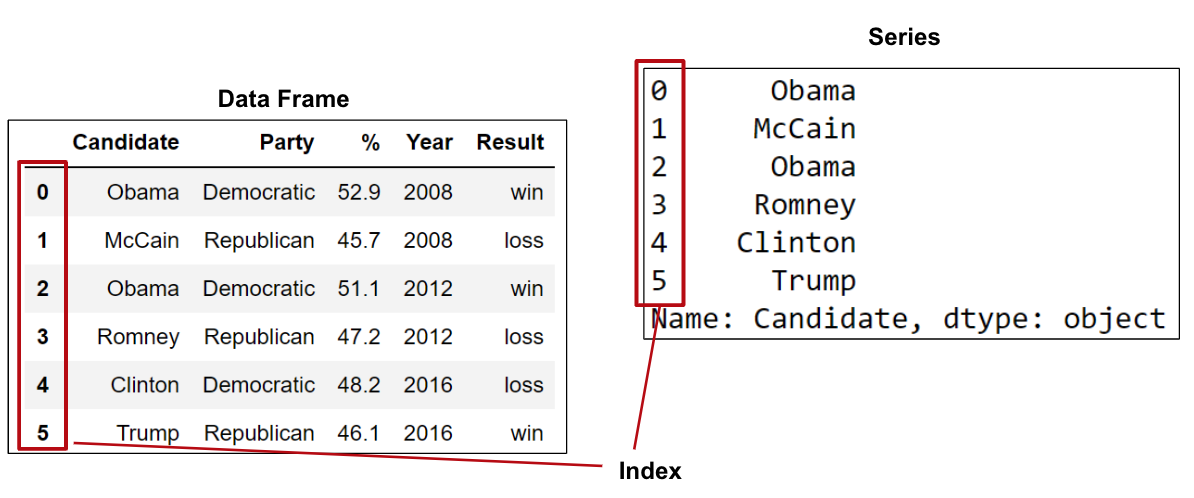
\includegraphics{pandas_1/images/df_series_index.png}

Notice how the \textbf{DataFrame} is a two dimensional object -- it
contains both rows and columns. The \textbf{Series} above is a singular
column of this DataFrame, namely the \texttt{Candidate} column. Both
contain an \textbf{Index}, or a shared list of row labels (the integers
from 0 to 5, inclusive).

\hypertarget{series}{%
\subsection{Series}\label{series}}

A Series represents a column of a DataFrame; more generally, it can be
any 1-dimensional array-like object containing values of the same type
with associated data labels, called its index.

\begin{Shaded}
\begin{Highlighting}[]
\ImportTok{import}\NormalTok{ pandas }\ImportTok{as}\NormalTok{ pd}

\NormalTok{s }\OperatorTok{=}\NormalTok{ pd.Series([}\OperatorTok{{-}}\DecValTok{1}\NormalTok{, }\DecValTok{10}\NormalTok{, }\DecValTok{2}\NormalTok{])}
\BuiltInTok{print}\NormalTok{(s)}
\end{Highlighting}
\end{Shaded}

\begin{verbatim}
0    -1
1    10
2     2
dtype: int64
\end{verbatim}

\begin{Shaded}
\begin{Highlighting}[]
\NormalTok{s.array }\CommentTok{\# Data contained within the Series}
\end{Highlighting}
\end{Shaded}

\begin{verbatim}
<PandasArray>
[-1, 10, 2]
Length: 3, dtype: int64
\end{verbatim}

\begin{Shaded}
\begin{Highlighting}[]
\NormalTok{s.index }\CommentTok{\# The Index of the Series}
\end{Highlighting}
\end{Shaded}

\begin{verbatim}
RangeIndex(start=0, stop=3, step=1)
\end{verbatim}

By default, row indices in \texttt{pandas} are a sequential list of
integers beginning from 0. Optionally, a list of desired indices can be
passed to the \texttt{index} argument.

\begin{Shaded}
\begin{Highlighting}[]
\NormalTok{s }\OperatorTok{=}\NormalTok{ pd.Series([}\OperatorTok{{-}}\DecValTok{1}\NormalTok{, }\DecValTok{10}\NormalTok{, }\DecValTok{2}\NormalTok{], index }\OperatorTok{=}\NormalTok{ [}\StringTok{"a"}\NormalTok{, }\StringTok{"b"}\NormalTok{, }\StringTok{"c"}\NormalTok{])}
\BuiltInTok{print}\NormalTok{(s)}
\end{Highlighting}
\end{Shaded}

\begin{verbatim}
a    -1
b    10
c     2
dtype: int64
\end{verbatim}

Indices can also be changed after initialization.

\begin{Shaded}
\begin{Highlighting}[]
\NormalTok{s.index }\OperatorTok{=}\NormalTok{ [}\StringTok{"first"}\NormalTok{, }\StringTok{"second"}\NormalTok{, }\StringTok{"third"}\NormalTok{]}
\BuiltInTok{print}\NormalTok{(s)}
\end{Highlighting}
\end{Shaded}

\begin{verbatim}
first     -1
second    10
third      2
dtype: int64
\end{verbatim}

\hypertarget{selection-in-series}{%
\subsubsection{Selection in Series}\label{selection-in-series}}

Similar to an array, we can select a single value or a set of values
from a Series. There are 3 primary methods of selecting data.

\begin{enumerate}
\def\labelenumi{\arabic{enumi}.}
\tightlist
\item
  A single index label
\item
  A list of index labels
\item
  A filtering condition
\end{enumerate}

Let's define the following Series \texttt{ser}

\begin{Shaded}
\begin{Highlighting}[]
\NormalTok{ser }\OperatorTok{=}\NormalTok{ pd.Series([}\DecValTok{4}\NormalTok{, }\OperatorTok{{-}}\DecValTok{2}\NormalTok{, }\DecValTok{0}\NormalTok{, }\DecValTok{6}\NormalTok{], index }\OperatorTok{=}\NormalTok{ [}\StringTok{"a"}\NormalTok{, }\StringTok{"b"}\NormalTok{, }\StringTok{"c"}\NormalTok{, }\StringTok{"d"}\NormalTok{])}
\BuiltInTok{print}\NormalTok{(ser)}
\end{Highlighting}
\end{Shaded}

\begin{verbatim}
a    4
b   -2
c    0
d    6
dtype: int64
\end{verbatim}

\hypertarget{a-single-index-label}{%
\paragraph{A Single Index Label}\label{a-single-index-label}}

\begin{Shaded}
\begin{Highlighting}[]
\NormalTok{ser[}\StringTok{"a"}\NormalTok{] }\CommentTok{\# Notice how the return value is a single array element}
\end{Highlighting}
\end{Shaded}

\begin{verbatim}
4
\end{verbatim}

\hypertarget{a-list-of-index-labels}{%
\paragraph{A List of Index Labels}\label{a-list-of-index-labels}}

\begin{Shaded}
\begin{Highlighting}[]
\NormalTok{ser[[}\StringTok{"a"}\NormalTok{, }\StringTok{"c"}\NormalTok{]] }\CommentTok{\# Notice how the return value is another Series}
\end{Highlighting}
\end{Shaded}

\begin{tabular}{lr}
\toprule
{} &  0 \\
\midrule
a &  4 \\
c &  0 \\
\bottomrule
\end{tabular}

\hypertarget{a-filtering-condition}{%
\paragraph{A Filtering Condition}\label{a-filtering-condition}}

Perhaps the most interesting (and useful) method of selecting data from
a Series is with a filtering condition.

We first must apply a vectorized boolean operation to our Series that
encodes the filter conditon.

\begin{Shaded}
\begin{Highlighting}[]
\NormalTok{ser }\OperatorTok{\textgreater{}} \DecValTok{0} \CommentTok{\# Filter condition: select all elements greater than 0}
\end{Highlighting}
\end{Shaded}

\begin{tabular}{ll}
\toprule
{} &      0 \\
\midrule
a &   True \\
b &  False \\
c &  False \\
d &   True \\
\bottomrule
\end{tabular}

Upon ``indexing'' in our Series with this condition, \texttt{pandas}
selects only the rows with \texttt{True} values.

\begin{Shaded}
\begin{Highlighting}[]
\NormalTok{ser[ser }\OperatorTok{\textgreater{}} \DecValTok{0}\NormalTok{] }
\end{Highlighting}
\end{Shaded}

\begin{tabular}{lr}
\toprule
{} &  0 \\
\midrule
a &  4 \\
d &  6 \\
\bottomrule
\end{tabular}

\hypertarget{dataframes}{%
\subsection{DataFrames}\label{dataframes}}

In Data 8, you encountered the \texttt{Table} class of the
\texttt{datascience} library, which represented tabular data. In Data
100, we'll be using the \texttt{DataFrame} class of the \texttt{pandas}
library.

Here is an example of a DataFrame that contains election data.

\begin{Shaded}
\begin{Highlighting}[]
\ImportTok{import}\NormalTok{ pandas }\ImportTok{as}\NormalTok{ pd}

\NormalTok{elections }\OperatorTok{=}\NormalTok{ pd.read\_csv(}\StringTok{"data/elections.csv"}\NormalTok{)}
\NormalTok{elections}
\end{Highlighting}
\end{Shaded}

\begin{tabular}{lrllrlr}
\toprule
{} &  Year &               Candidate &                  Party &  Popular vote & Result &          \% \\
\midrule
0   &  1824 &          Andrew Jackson &  Democratic-Republican &        151271 &   loss &  57.210122 \\
1   &  1824 &       John Quincy Adams &  Democratic-Republican &        113142 &    win &  42.789878 \\
2   &  1828 &          Andrew Jackson &             Democratic &        642806 &    win &  56.203927 \\
3   &  1828 &       John Quincy Adams &    National Republican &        500897 &   loss &  43.796073 \\
4   &  1832 &          Andrew Jackson &             Democratic &        702735 &    win &  54.574789 \\
5   &  1832 &              Henry Clay &    National Republican &        484205 &   loss &  37.603628 \\
6   &  1832 &            William Wirt &           Anti-Masonic &        100715 &   loss &   7.821583 \\
7   &  1836 &       Hugh Lawson White &                   Whig &        146109 &   loss &  10.005985 \\
8   &  1836 &        Martin Van Buren &             Democratic &        763291 &    win &  52.272472 \\
9   &  1836 &  William Henry Harrison &                   Whig &        550816 &   loss &  37.721543 \\
10  &  1840 &        Martin Van Buren &             Democratic &       1128854 &   loss &  46.948787 \\
11  &  1840 &  William Henry Harrison &                   Whig &       1275583 &    win &  53.051213 \\
12  &  1844 &              Henry Clay &                   Whig &       1300004 &   loss &  49.250523 \\
13  &  1844 &              James Polk &             Democratic &       1339570 &    win &  50.749477 \\
14  &  1848 &              Lewis Cass &             Democratic &       1223460 &   loss &  42.552229 \\
15  &  1848 &        Martin Van Buren &              Free Soil &        291501 &   loss &  10.138474 \\
16  &  1848 &          Zachary Taylor &                   Whig &       1360235 &    win &  47.309296 \\
17  &  1852 &         Franklin Pierce &             Democratic &       1605943 &    win &  51.013168 \\
18  &  1852 &            John P. Hale &              Free Soil &        155210 &   loss &   4.930283 \\
19  &  1852 &          Winfield Scott &                   Whig &       1386942 &   loss &  44.056548 \\
20  &  1856 &          James Buchanan &             Democratic &       1835140 &    win &  45.306080 \\
21  &  1856 &         John C. Frémont &             Republican &       1342345 &   loss &  33.139919 \\
22  &  1856 &        Millard Fillmore &               American &        873053 &   loss &  21.554001 \\
23  &  1860 &         Abraham Lincoln &             Republican &       1855993 &    win &  39.699408 \\
24  &  1860 &               John Bell &   Constitutional Union &        590901 &   loss &  12.639283 \\
25  &  1860 &    John C. Breckinridge &    Southern Democratic &        848019 &   loss &  18.138998 \\
26  &  1860 &      Stephen A. Douglas &    Northern Democratic &       1380202 &   loss &  29.522311 \\
27  &  1864 &         Abraham Lincoln &         National Union &       2211317 &    win &  54.951512 \\
28  &  1864 &     George B. McClellan &             Democratic &       1812807 &   loss &  45.048488 \\
29  &  1868 &         Horatio Seymour &             Democratic &       2708744 &   loss &  47.334695 \\
30  &  1868 &           Ulysses Grant &             Republican &       3013790 &    win &  52.665305 \\
31  &  1872 &          Horace Greeley &     Liberal Republican &       2834761 &   loss &  44.071406 \\
32  &  1872 &           Ulysses Grant &             Republican &       3597439 &    win &  55.928594 \\
33  &  1876 &        Rutherford Hayes &             Republican &       4034142 &    win &  48.471624 \\
34  &  1876 &        Samuel J. Tilden &             Democratic &       4288546 &   loss &  51.528376 \\
35  &  1880 &         James B. Weaver &              Greenback &        308649 &   loss &   3.352344 \\
36  &  1880 &          James Garfield &             Republican &       4453337 &    win &  48.369234 \\
37  &  1880 &  Winfield Scott Hancock &             Democratic &       4444976 &   loss &  48.278422 \\
38  &  1884 &         Benjamin Butler &          Anti-Monopoly &        134294 &   loss &   1.335838 \\
39  &  1884 &        Grover Cleveland &             Democratic &       4914482 &    win &  48.884933 \\
40  &  1884 &         James G. Blaine &             Republican &       4856905 &   loss &  48.312208 \\
41  &  1884 &           John St. John &            Prohibition &        147482 &   loss &   1.467021 \\
42  &  1888 &          Alson Streeter &            Union Labor &        146602 &   loss &   1.288861 \\
43  &  1888 &       Benjamin Harrison &             Republican &       5443633 &    win &  47.858041 \\
44  &  1888 &         Clinton B. Fisk &            Prohibition &        249819 &   loss &   2.196299 \\
45  &  1888 &        Grover Cleveland &             Democratic &       5534488 &   loss &  48.656799 \\
46  &  1892 &       Benjamin Harrison &             Republican &       5176108 &   loss &  42.984101 \\
47  &  1892 &        Grover Cleveland &             Democratic &       5553898 &    win &  46.121393 \\
48  &  1892 &         James B. Weaver &               Populist &       1041028 &   loss &   8.645038 \\
49  &  1892 &            John Bidwell &            Prohibition &        270879 &   loss &   2.249468 \\
50  &  1896 &          John M. Palmer &    National Democratic &        134645 &   loss &   0.969566 \\
51  &  1896 &         Joshua Levering &            Prohibition &        131312 &   loss &   0.945565 \\
52  &  1896 &  William Jennings Bryan &             Democratic &       6509052 &   loss &  46.871053 \\
53  &  1896 &        William McKinley &             Republican &       7112138 &    win &  51.213817 \\
54  &  1900 &         John G. Woolley &            Prohibition &        210864 &   loss &   1.526821 \\
55  &  1900 &  William Jennings Bryan &             Democratic &       6370932 &   loss &  46.130540 \\
56  &  1900 &        William McKinley &             Republican &       7228864 &    win &  52.342640 \\
57  &  1904 &         Alton B. Parker &             Democratic &       5083880 &   loss &  37.685116 \\
58  &  1904 &          Eugene V. Debs &              Socialist &        402810 &   loss &   2.985897 \\
59  &  1904 &        Silas C. Swallow &            Prohibition &        259102 &   loss &   1.920637 \\
60  &  1904 &      Theodore Roosevelt &             Republican &       7630557 &    win &  56.562787 \\
61  &  1904 &        Thomas E. Watson &               Populist &        114070 &   loss &   0.845563 \\
62  &  1908 &          Eugene V. Debs &              Socialist &        420852 &   loss &   2.850866 \\
63  &  1908 &        Eugene W. Chafin &            Prohibition &        254087 &   loss &   1.721194 \\
64  &  1908 &  William Jennings Bryan &             Democratic &       6408979 &   loss &  43.414640 \\
65  &  1908 &            William Taft &             Republican &       7678335 &    win &  52.013300 \\
66  &  1912 &          Eugene V. Debs &              Socialist &        901551 &   loss &   6.004354 \\
67  &  1912 &        Eugene W. Chafin &            Prohibition &        208156 &   loss &   1.386325 \\
68  &  1912 &      Theodore Roosevelt &            Progressive &       4122721 &   loss &  27.457433 \\
69  &  1912 &            William Taft &             Republican &       3486242 &   loss &  23.218466 \\
70  &  1912 &          Woodrow Wilson &             Democratic &       6296284 &    win &  41.933422 \\
71  &  1916 &         Allan L. Benson &              Socialist &        590524 &   loss &   3.194193 \\
72  &  1916 &    Charles Evans Hughes &             Republican &       8548728 &   loss &  46.240779 \\
73  &  1916 &             Frank Hanly &            Prohibition &        221302 &   loss &   1.197041 \\
74  &  1916 &          Woodrow Wilson &             Democratic &       9126868 &    win &  49.367987 \\
75  &  1920 &        Aaron S. Watkins &            Prohibition &        188787 &   loss &   0.708351 \\
76  &  1920 &          Eugene V. Debs &              Socialist &        913693 &   loss &   3.428282 \\
77  &  1920 &            James M. Cox &             Democratic &       9139661 &   loss &  34.293063 \\
78  &  1920 &   Parley P. Christensen &           Farmer–Labor &        265398 &   loss &   0.995804 \\
79  &  1920 &          Warren Harding &             Republican &      16144093 &    win &  60.574501 \\
80  &  1924 &         Calvin Coolidge &             Republican &      15723789 &    win &  54.329113 \\
81  &  1924 &           John W. Davis &             Democratic &       8386242 &   loss &  28.976291 \\
82  &  1924 &      Robert La Follette &            Progressive &       4831706 &   loss &  16.694596 \\
83  &  1928 &                Al Smith &             Democratic &      15015464 &   loss &  40.902853 \\
84  &  1928 &          Herbert Hoover &             Republican &      21427123 &    win &  58.368524 \\
85  &  1928 &           Norman Thomas &              Socialist &        267478 &   loss &   0.728623 \\
86  &  1932 &      Franklin Roosevelt &             Democratic &      22821277 &    win &  57.672125 \\
87  &  1932 &          Herbert Hoover &             Republican &      15761254 &   loss &  39.830594 \\
88  &  1932 &           Norman Thomas &              Socialist &        884885 &   loss &   2.236211 \\
89  &  1932 &       William Z. Foster &              Communist &        103307 &   loss &   0.261069 \\
90  &  1936 &              Alf Landon &             Republican &      16679543 &   loss &  36.648285 \\
91  &  1936 &      Franklin Roosevelt &             Democratic &      27752648 &    win &  60.978107 \\
92  &  1936 &           Norman Thomas &              Socialist &        187910 &   loss &   0.412876 \\
93  &  1936 &           William Lemke &                  Union &        892378 &   loss &   1.960733 \\
94  &  1940 &      Franklin Roosevelt &             Democratic &      27313945 &    win &  54.871202 \\
95  &  1940 &           Norman Thomas &              Socialist &        116599 &   loss &   0.234237 \\
96  &  1940 &         Wendell Willkie &             Republican &      22347744 &   loss &  44.894561 \\
97  &  1944 &      Franklin Roosevelt &             Democratic &      25612916 &    win &  53.773801 \\
98  &  1944 &         Thomas E. Dewey &             Republican &      22017929 &   loss &  46.226199 \\
99  &  1948 &        Claude A. Watson &            Prohibition &        103708 &   loss &   0.212747 \\
100 &  1948 &            Harry Truman &             Democratic &      24179347 &    win &  49.601536 \\
101 &  1948 &        Henry A. Wallace &            Progressive &       1157328 &   loss &   2.374144 \\
102 &  1948 &           Norman Thomas &              Socialist &        139569 &   loss &   0.286312 \\
103 &  1948 &          Strom Thurmond &              Dixiecrat &       1175930 &   loss &   2.412304 \\
104 &  1948 &         Thomas E. Dewey &             Republican &      21991292 &   loss &  45.112958 \\
105 &  1952 &         Adlai Stevenson &             Democratic &      27375090 &   loss &  44.446312 \\
106 &  1952 &       Dwight Eisenhower &             Republican &      34075529 &    win &  55.325173 \\
107 &  1952 &        Vincent Hallinan &            Progressive &        140746 &   loss &   0.228516 \\
108 &  1956 &         Adlai Stevenson &             Democratic &      26028028 &   loss &  42.174464 \\
109 &  1956 &       Dwight Eisenhower &             Republican &      35579180 &    win &  57.650654 \\
110 &  1956 &      T. Coleman Andrews &         States' Rights &        107929 &   loss &   0.174883 \\
111 &  1960 &            John Kennedy &             Democratic &      34220984 &    win &  50.082561 \\
112 &  1960 &           Richard Nixon &             Republican &      34108157 &   loss &  49.917439 \\
113 &  1964 &         Barry Goldwater &             Republican &      27175754 &   loss &  38.655297 \\
114 &  1964 &          Lyndon Johnson &             Democratic &      43127041 &    win &  61.344703 \\
115 &  1968 &          George Wallace &   American Independent &       9901118 &   loss &  13.571218 \\
116 &  1968 &         Hubert Humphrey &             Democratic &      31271839 &   loss &  42.863537 \\
117 &  1968 &           Richard Nixon &             Republican &      31783783 &    win &  43.565246 \\
118 &  1972 &         George McGovern &             Democratic &      29173222 &   loss &  37.670670 \\
119 &  1972 &         John G. Schmitz &   American Independent &       1100868 &   loss &   1.421524 \\
120 &  1972 &           Richard Nixon &             Republican &      47168710 &    win &  60.907806 \\
121 &  1976 &         Eugene McCarthy &            Independent &        740460 &   loss &   0.911649 \\
122 &  1976 &             Gerald Ford &             Republican &      39148634 &   loss &  48.199499 \\
123 &  1976 &            Jimmy Carter &             Democratic &      40831881 &    win &  50.271900 \\
124 &  1976 &           Lester Maddox &   American Independent &        170274 &   loss &   0.209640 \\
125 &  1976 &          Roger MacBride &            Libertarian &        172557 &   loss &   0.212451 \\
126 &  1976 &      Thomas J. Anderson &               American &        158271 &   loss &   0.194862 \\
127 &  1980 &          Barry Commoner &               Citizens &        233052 &   loss &   0.270182 \\
128 &  1980 &                Ed Clark &            Libertarian &        921128 &   loss &   1.067883 \\
129 &  1980 &            Jimmy Carter &             Democratic &      35480115 &   loss &  41.132848 \\
130 &  1980 &        John B. Anderson &            Independent &       5719850 &   loss &   6.631143 \\
131 &  1980 &           Ronald Reagan &             Republican &      43903230 &    win &  50.897944 \\
132 &  1984 &          David Bergland &            Libertarian &        228111 &   loss &   0.247245 \\
133 &  1984 &           Ronald Reagan &             Republican &      54455472 &    win &  59.023326 \\
134 &  1984 &          Walter Mondale &             Democratic &      37577352 &   loss &  40.729429 \\
135 &  1988 &       George H. W. Bush &             Republican &      48886597 &    win &  53.518845 \\
136 &  1988 &           Lenora Fulani &           New Alliance &        217221 &   loss &   0.237804 \\
137 &  1988 &         Michael Dukakis &             Democratic &      41809074 &   loss &  45.770691 \\
138 &  1988 &                Ron Paul &            Libertarian &        431750 &   loss &   0.472660 \\
139 &  1992 &            Andre Marrou &            Libertarian &        290087 &   loss &   0.278516 \\
140 &  1992 &            Bill Clinton &             Democratic &      44909806 &    win &  43.118485 \\
141 &  1992 &                Bo Gritz &               Populist &        106152 &   loss &   0.101918 \\
142 &  1992 &       George H. W. Bush &             Republican &      39104550 &   loss &  37.544784 \\
143 &  1992 &              Ross Perot &            Independent &      19743821 &   loss &  18.956298 \\
144 &  1996 &            Bill Clinton &             Democratic &      47400125 &    win &  49.296938 \\
145 &  1996 &                Bob Dole &             Republican &      39197469 &   loss &  40.766036 \\
146 &  1996 &            Harry Browne &            Libertarian &        485759 &   loss &   0.505198 \\
147 &  1996 &         Howard Phillips &              Taxpayers &        184656 &   loss &   0.192045 \\
148 &  1996 &            John Hagelin &            Natural Law &        113670 &   loss &   0.118219 \\
149 &  1996 &             Ralph Nader &                  Green &        685297 &   loss &   0.712721 \\
150 &  1996 &              Ross Perot &                 Reform &       8085294 &   loss &   8.408844 \\
151 &  2000 &                 Al Gore &             Democratic &      50999897 &   loss &  48.491813 \\
152 &  2000 &          George W. Bush &             Republican &      50456002 &    win &  47.974666 \\
153 &  2000 &            Harry Browne &            Libertarian &        384431 &   loss &   0.365525 \\
154 &  2000 &            Pat Buchanan &                 Reform &        448895 &   loss &   0.426819 \\
155 &  2000 &             Ralph Nader &                  Green &       2882955 &   loss &   2.741176 \\
156 &  2004 &              David Cobb &                  Green &        119859 &   loss &   0.098088 \\
157 &  2004 &          George W. Bush &             Republican &      62040610 &    win &  50.771824 \\
158 &  2004 &              John Kerry &             Democratic &      59028444 &   loss &  48.306775 \\
159 &  2004 &        Michael Badnarik &            Libertarian &        397265 &   loss &   0.325108 \\
160 &  2004 &        Michael Peroutka &           Constitution &        143630 &   loss &   0.117542 \\
161 &  2004 &             Ralph Nader &            Independent &        465151 &   loss &   0.380663 \\
162 &  2008 &            Barack Obama &             Democratic &      69498516 &    win &  53.023510 \\
163 &  2008 &                Bob Barr &            Libertarian &        523715 &   loss &   0.399565 \\
164 &  2008 &           Chuck Baldwin &           Constitution &        199750 &   loss &   0.152398 \\
165 &  2008 &        Cynthia McKinney &                  Green &        161797 &   loss &   0.123442 \\
166 &  2008 &             John McCain &             Republican &      59948323 &   loss &  45.737243 \\
167 &  2008 &             Ralph Nader &            Independent &        739034 &   loss &   0.563842 \\
168 &  2012 &            Barack Obama &             Democratic &      65915795 &    win &  51.258484 \\
169 &  2012 &            Gary Johnson &            Libertarian &       1275971 &   loss &   0.992241 \\
170 &  2012 &              Jill Stein &                  Green &        469627 &   loss &   0.365199 \\
171 &  2012 &             Mitt Romney &             Republican &      60933504 &   loss &  47.384076 \\
172 &  2016 &          Darrell Castle &           Constitution &        203091 &   loss &   0.149640 \\
173 &  2016 &            Donald Trump &             Republican &      62984828 &    win &  46.407862 \\
174 &  2016 &           Evan McMullin &            Independent &        732273 &   loss &   0.539546 \\
175 &  2016 &            Gary Johnson &            Libertarian &       4489235 &   loss &   3.307714 \\
176 &  2016 &         Hillary Clinton &             Democratic &      65853514 &   loss &  48.521539 \\
177 &  2016 &              Jill Stein &                  Green &       1457226 &   loss &   1.073699 \\
178 &  2020 &            Joseph Biden &             Democratic &      81268924 &    win &  51.311515 \\
179 &  2020 &            Donald Trump &             Republican &      74216154 &   loss &  46.858542 \\
180 &  2020 &            Jo Jorgensen &            Libertarian &       1865724 &   loss &   1.177979 \\
181 &  2020 &          Howard Hawkins &                  Green &        405035 &   loss &   0.255731 \\
\bottomrule
\end{tabular}

Let's dissect the code above.

\begin{enumerate}
\def\labelenumi{\arabic{enumi}.}
\item
  We first import the \texttt{pandas} library into our Python
  environment, using the alias \texttt{pd}.
   \texttt{import\ pandas\ as\ pd}
\item
  There are a number of ways to read data into a DataFrame. In Data 100,
  our data are typically stored in a CSV (comma-seperated values) file
  format. We can import a CSV file into a DataFrame by passing the data
  path as an argument to the following \texttt{pandas} function.
   \texttt{pd.read\_csv("elections.csv")}
\end{enumerate}

This code stores our DataFrame object in the \texttt{elections}
variable. Upon inspection, our \texttt{elections} DataFrame has 182 rows
and 6 columns (\texttt{Year}, \texttt{Candidate}, \texttt{Party},
\texttt{Popular\ Vote}, \texttt{Result}, \texttt{\%}). Each row
represents a single record -- in our example, a presedential candidate
from some particular year. Each column represents a single attribute, or
feature of the record.

In the example above, we constructed a DataFrame object using data from
a CSV file. As we'll explore in the next section, we can create a
DataFrame with data of our own.

\hypertarget{creating-a-dataframe}{%
\subsubsection{Creating a DataFrame}\label{creating-a-dataframe}}

There are many ways to create a DataFrame. Here, we will cover the most
popular approaches.

\begin{enumerate}
\def\labelenumi{\arabic{enumi}.}
\tightlist
\item
  Using a list and column names
\item
  From a dictionary
\item
  From a Series
\end{enumerate}

\hypertarget{using-a-list-and-column-names}{%
\paragraph{Using a List and Column
Names}\label{using-a-list-and-column-names}}

Consider the following examples.

\begin{Shaded}
\begin{Highlighting}[]
\NormalTok{df\_list }\OperatorTok{=}\NormalTok{ pd.DataFrame([}\DecValTok{1}\NormalTok{, }\DecValTok{2}\NormalTok{, }\DecValTok{3}\NormalTok{], columns}\OperatorTok{=}\NormalTok{[}\StringTok{"Numbers"}\NormalTok{])}
\NormalTok{df\_list}
\end{Highlighting}
\end{Shaded}

\begin{tabular}{lr}
\toprule
{} &  Numbers \\
\midrule
0 &        1 \\
1 &        2 \\
2 &        3 \\
\bottomrule
\end{tabular}

The first code cell creates a DataFrame with a single column
\texttt{Numbers}, while the second creates a DataFrame with an
additional column \texttt{Description}. Notice how a 2D list of values
is required to initialize the second DataFrame -- each nested list
represents a single row of data.

\begin{Shaded}
\begin{Highlighting}[]
\NormalTok{df\_list }\OperatorTok{=}\NormalTok{ pd.DataFrame([[}\DecValTok{1}\NormalTok{, }\StringTok{"one"}\NormalTok{], [}\DecValTok{2}\NormalTok{, }\StringTok{"two"}\NormalTok{]], columns }\OperatorTok{=}\NormalTok{ [}\StringTok{"Number"}\NormalTok{, }\StringTok{"Description"}\NormalTok{])}
\NormalTok{df\_list}
\end{Highlighting}
\end{Shaded}

\begin{tabular}{lrl}
\toprule
{} &  Number & Description \\
\midrule
0 &       1 &         one \\
1 &       2 &         two \\
\bottomrule
\end{tabular}

\hypertarget{from-a-dictionary}{%
\paragraph{From a Dictionary}\label{from-a-dictionary}}

A second (and more common) way to create a DataFrame is with a
dictionary. The dictionary keys represent the column names, and the
dictionary values represent the column values.

\begin{Shaded}
\begin{Highlighting}[]
\NormalTok{df\_dict }\OperatorTok{=}\NormalTok{ pd.DataFrame(\{}\StringTok{"Fruit"}\NormalTok{: [}\StringTok{"Strawberry"}\NormalTok{, }\StringTok{"Orange"}\NormalTok{], }\StringTok{"Price"}\NormalTok{: [}\FloatTok{5.49}\NormalTok{, }\FloatTok{3.99}\NormalTok{]\})}
\NormalTok{df\_dict}
\end{Highlighting}
\end{Shaded}

\begin{tabular}{llr}
\toprule
{} &       Fruit &  Price \\
\midrule
0 &  Strawberry &   5.49 \\
1 &      Orange &   3.99 \\
\bottomrule
\end{tabular}

\hypertarget{from-a-series}{%
\paragraph{From a Series}\label{from-a-series}}

Earlier, we explained how a Series was synonymous to a column in a
DataFrame. It follows then, that a DataFrame is equivalent to a
collection of Series, which all share the same index.

In fact, we can initialize a DataFrame by merging two or more Series.

\begin{Shaded}
\begin{Highlighting}[]
\CommentTok{\# Notice how our indices, or row labels, are the same}

\NormalTok{s\_a }\OperatorTok{=}\NormalTok{ pd.Series([}\StringTok{"a1"}\NormalTok{, }\StringTok{"a2"}\NormalTok{, }\StringTok{"a3"}\NormalTok{], index }\OperatorTok{=}\NormalTok{ [}\StringTok{"r1"}\NormalTok{, }\StringTok{"r2"}\NormalTok{, }\StringTok{"r3"}\NormalTok{])}
\NormalTok{s\_b }\OperatorTok{=}\NormalTok{ pd.Series([}\StringTok{"b1"}\NormalTok{, }\StringTok{"b2"}\NormalTok{, }\StringTok{"b3"}\NormalTok{], index }\OperatorTok{=}\NormalTok{ [}\StringTok{"r1"}\NormalTok{, }\StringTok{"r2"}\NormalTok{, }\StringTok{"r3"}\NormalTok{])}

\NormalTok{pd.DataFrame(\{}\StringTok{"A{-}column"}\NormalTok{: s\_a, }\StringTok{"B{-}column"}\NormalTok{: s\_b\})}
\end{Highlighting}
\end{Shaded}

\begin{tabular}{lll}
\toprule
{} & A-column & B-column \\
\midrule
r1 &       a1 &       b1 \\
r2 &       a2 &       b2 \\
r3 &       a3 &       b3 \\
\bottomrule
\end{tabular}

\hypertarget{indices}{%
\subsection{Indices}\label{indices}}

The major takeaway: we can think of a \textbf{DataFrame} as a collection
of \textbf{Series} that all share the same \textbf{Index}.

On a more technical note, an Index doesn't have to be an integer, nor
does it have to be unique. For example, we can set the index of the
\texttt{elections} Dataframe to be the name of presedential candidates.
Selecting a new Series from this modified DataFrame yields the
following.

\begin{Shaded}
\begin{Highlighting}[]
\CommentTok{\# This sets the index to the "Candidate" column}
\NormalTok{elections.set\_index(}\StringTok{"Candidate"}\NormalTok{, inplace}\OperatorTok{=}\VariableTok{True}\NormalTok{)}
\end{Highlighting}
\end{Shaded}

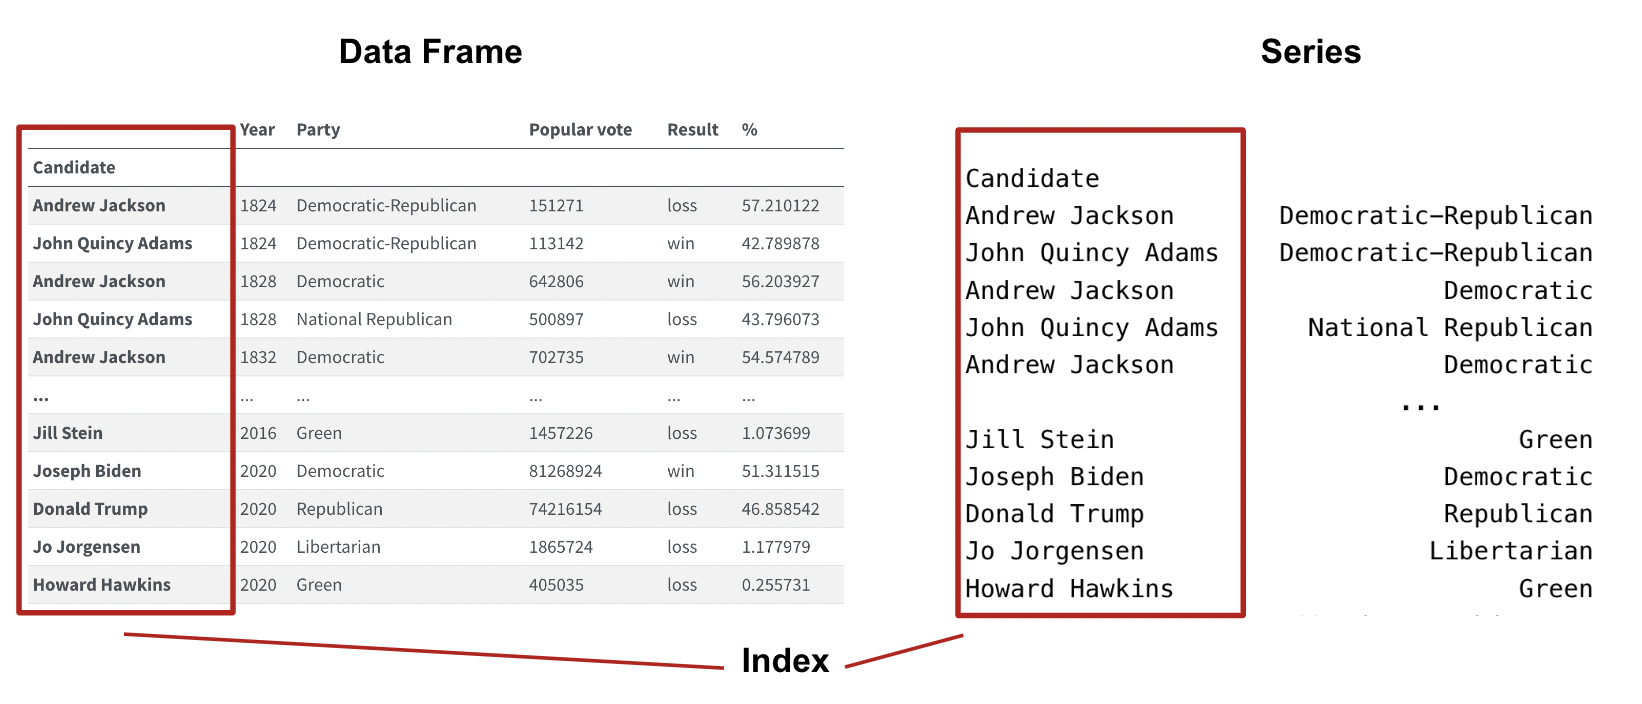
\includegraphics{pandas_1/images/index_comparison_2.png}

To retrieve the indices of a DataFrame, simply use the \texttt{.index}
attribute of the DataFrame class.

\begin{Shaded}
\begin{Highlighting}[]
\NormalTok{elections.index}
\end{Highlighting}
\end{Shaded}

\begin{verbatim}
Index(['Andrew Jackson', 'John Quincy Adams', 'Andrew Jackson',
       'John Quincy Adams', 'Andrew Jackson', 'Henry Clay', 'William Wirt',
       'Hugh Lawson White', 'Martin Van Buren', 'William Henry Harrison',
       ...
       'Darrell Castle', 'Donald Trump', 'Evan McMullin', 'Gary Johnson',
       'Hillary Clinton', 'Jill Stein', 'Joseph Biden', 'Donald Trump',
       'Jo Jorgensen', 'Howard Hawkins'],
      dtype='object', name='Candidate', length=182)
\end{verbatim}

\begin{Shaded}
\begin{Highlighting}[]
\CommentTok{\# This resets the index to be the default list of integers}
\NormalTok{elections.reset\_index(inplace}\OperatorTok{=}\VariableTok{True}\NormalTok{) }
\end{Highlighting}
\end{Shaded}

\hypertarget{slicing-in-dataframes}{%
\section{Slicing in DataFrames}\label{slicing-in-dataframes}}

Now that we've learned how to create DataFrames, let's dive deeper into
their capabilities.

The API (application programming interface) for the DataFrame class is
enormous. In this section, we'll discuss several methods of the
DataFrame API that allow us to extract subsets of data.

The simplest way to manipulate a DataFrame is to extract a subset of
rows and columns, known as \textbf{slicing}. We will do so with three
primary methods of the DataFrame class:

\begin{enumerate}
\def\labelenumi{\arabic{enumi}.}
\tightlist
\item
  \texttt{.loc}
\item
  \texttt{.iloc}
\item
  \texttt{{[}{]}}
\end{enumerate}

\hypertarget{indexing-with-.loc}{%
\subsection{Indexing with .loc}\label{indexing-with-.loc}}

The \texttt{.loc} operator selects rows and columns in a DataFrame by
their row and column label(s), respectively. The \textbf{row labels}
(commonly referred to as the \textbf{indices}) are the bold text on the
far \emph{left} of a DataFrame, while the \textbf{column labels} are the
column names found at the \emph{top} of a DataFrame.

To grab data with \texttt{.loc}, we must specify the row and column
label(s) where the data exists. The row labels are the first argument to
the \texttt{.loc} function; the column labels are the second. For
example, we can select the the row labeled \texttt{0} and the column
labeled \texttt{Candidate} from the \texttt{elections} DataFrame.

\begin{Shaded}
\begin{Highlighting}[]
\NormalTok{elections.loc[}\DecValTok{0}\NormalTok{, }\StringTok{\textquotesingle{}Candidate\textquotesingle{}}\NormalTok{]}
\end{Highlighting}
\end{Shaded}

\begin{verbatim}
'Andrew Jackson'
\end{verbatim}

To select \emph{multiple} rows and columns, we can use Python slice
notation. Here, we select both the first four rows and columns.

\begin{Shaded}
\begin{Highlighting}[]
\NormalTok{elections.loc[}\DecValTok{0}\NormalTok{:}\DecValTok{3}\NormalTok{, }\StringTok{\textquotesingle{}Year\textquotesingle{}}\NormalTok{:}\StringTok{\textquotesingle{}Popular vote\textquotesingle{}}\NormalTok{]}
\end{Highlighting}
\end{Shaded}

\begin{tabular}{lrlr}
\toprule
{} &  Year &                  Party &  Popular vote \\
\midrule
0 &  1824 &  Democratic-Republican &        151271 \\
1 &  1824 &  Democratic-Republican &        113142 \\
2 &  1828 &             Democratic &        642806 \\
3 &  1828 &    National Republican &        500897 \\
\bottomrule
\end{tabular}

Suppose that instead, we wanted \emph{every} column value for the first
four rows in the \texttt{elections} DataFrame. The shorthand \texttt{:}
is useful for this.

\begin{Shaded}
\begin{Highlighting}[]
\NormalTok{elections.loc[}\DecValTok{0}\NormalTok{:}\DecValTok{3}\NormalTok{, :]}
\end{Highlighting}
\end{Shaded}

\begin{tabular}{llrlrlr}
\toprule
{} &          Candidate &  Year &                  Party &  Popular vote & Result &          \% \\
\midrule
0 &     Andrew Jackson &  1824 &  Democratic-Republican &        151271 &   loss &  57.210122 \\
1 &  John Quincy Adams &  1824 &  Democratic-Republican &        113142 &    win &  42.789878 \\
2 &     Andrew Jackson &  1828 &             Democratic &        642806 &    win &  56.203927 \\
3 &  John Quincy Adams &  1828 &    National Republican &        500897 &   loss &  43.796073 \\
\bottomrule
\end{tabular}

There are a couple of things we should note. Unlike conventional Python,
Pandas allows us to slice string values (in our example, the column
labels). Secondly, slicing with \texttt{.loc} is \emph{inclusive}.
Notice how our resulting DataFrame includes every row and column between
and including the slice labels we specified.

Equivalently, we can use a list to obtain multiple rows and columns in
our \texttt{elections} DataFrame.

\begin{Shaded}
\begin{Highlighting}[]
\NormalTok{elections.loc[[}\DecValTok{0}\NormalTok{, }\DecValTok{1}\NormalTok{, }\DecValTok{2}\NormalTok{, }\DecValTok{3}\NormalTok{], [}\StringTok{\textquotesingle{}Year\textquotesingle{}}\NormalTok{, }\StringTok{\textquotesingle{}Candidate\textquotesingle{}}\NormalTok{, }\StringTok{\textquotesingle{}Party\textquotesingle{}}\NormalTok{, }\StringTok{\textquotesingle{}Popular vote\textquotesingle{}}\NormalTok{]]}
\end{Highlighting}
\end{Shaded}

\begin{tabular}{lrllr}
\toprule
{} &  Year &          Candidate &                  Party &  Popular vote \\
\midrule
0 &  1824 &     Andrew Jackson &  Democratic-Republican &        151271 \\
1 &  1824 &  John Quincy Adams &  Democratic-Republican &        113142 \\
2 &  1828 &     Andrew Jackson &             Democratic &        642806 \\
3 &  1828 &  John Quincy Adams &    National Republican &        500897 \\
\bottomrule
\end{tabular}

Lastly, we can interchange list and slicing notation.

\begin{Shaded}
\begin{Highlighting}[]
\NormalTok{elections.loc[[}\DecValTok{0}\NormalTok{, }\DecValTok{1}\NormalTok{, }\DecValTok{2}\NormalTok{, }\DecValTok{3}\NormalTok{], :]}
\end{Highlighting}
\end{Shaded}

\begin{tabular}{llrlrlr}
\toprule
{} &          Candidate &  Year &                  Party &  Popular vote & Result &          \% \\
\midrule
0 &     Andrew Jackson &  1824 &  Democratic-Republican &        151271 &   loss &  57.210122 \\
1 &  John Quincy Adams &  1824 &  Democratic-Republican &        113142 &    win &  42.789878 \\
2 &     Andrew Jackson &  1828 &             Democratic &        642806 &    win &  56.203927 \\
3 &  John Quincy Adams &  1828 &    National Republican &        500897 &   loss &  43.796073 \\
\bottomrule
\end{tabular}

\hypertarget{indexing-with-.iloc}{%
\subsection{Indexing with .iloc}\label{indexing-with-.iloc}}

Slicing with \texttt{.iloc} works similarily to \texttt{.loc}, although
\texttt{.iloc} uses the integer positions of rows and columns rather the
labels. The arguments to the \texttt{.iloc} function also behave
similarly - single values, lists, indices, and any combination of these
are permitted.

Let's begin reproducing our results from above. We'll begin by selecting
for the first presedential candidate in our \texttt{elections}
DataFrame:

\begin{Shaded}
\begin{Highlighting}[]
\CommentTok{\# elections.loc[0, "Candidate"] {-} Previous approach}
\NormalTok{elections.iloc[}\DecValTok{0}\NormalTok{, }\DecValTok{1}\NormalTok{]}
\end{Highlighting}
\end{Shaded}

\begin{verbatim}
1824
\end{verbatim}

Notice how the first argument to both \texttt{.loc} and \texttt{.iloc}
are the same. This is because the row with a label of 0 is conveniently
in the 0\textsuperscript{th} (or first) position of the
\texttt{elections} DataFrame. Generally, this is true of any DataFrame
where the row labels are incremented in ascending order from 0.

However, when we select the first four rows and columns using
\texttt{.iloc}, we notice something.

\begin{Shaded}
\begin{Highlighting}[]
\CommentTok{\# elections.loc[0:3, \textquotesingle{}Year\textquotesingle{}:\textquotesingle{}Popular vote\textquotesingle{}] {-} Previous approach}
\NormalTok{elections.iloc[}\DecValTok{0}\NormalTok{:}\DecValTok{4}\NormalTok{, }\DecValTok{0}\NormalTok{:}\DecValTok{4}\NormalTok{]}
\end{Highlighting}
\end{Shaded}

\begin{tabular}{llrlr}
\toprule
{} &          Candidate &  Year &                  Party &  Popular vote \\
\midrule
0 &     Andrew Jackson &  1824 &  Democratic-Republican &        151271 \\
1 &  John Quincy Adams &  1824 &  Democratic-Republican &        113142 \\
2 &     Andrew Jackson &  1828 &             Democratic &        642806 \\
3 &  John Quincy Adams &  1828 &    National Republican &        500897 \\
\bottomrule
\end{tabular}

Slicing is no longer inclusive in \texttt{.iloc} - it's
\emph{exclusive}. This is one of Pandas syntatical subtleties; you'll
get used to with practice.

List behavior works just as expected.

\begin{Shaded}
\begin{Highlighting}[]
\CommentTok{\#elections.loc[[0, 1, 2, 3], [\textquotesingle{}Year\textquotesingle{}, \textquotesingle{}Candidate\textquotesingle{}, \textquotesingle{}Party\textquotesingle{}, \textquotesingle{}Popular vote\textquotesingle{}]] {-} Previous Approach}
\NormalTok{elections.iloc[[}\DecValTok{0}\NormalTok{, }\DecValTok{1}\NormalTok{, }\DecValTok{2}\NormalTok{, }\DecValTok{3}\NormalTok{], [}\DecValTok{0}\NormalTok{, }\DecValTok{1}\NormalTok{, }\DecValTok{2}\NormalTok{, }\DecValTok{3}\NormalTok{]]}
\end{Highlighting}
\end{Shaded}

\begin{tabular}{llrlr}
\toprule
{} &          Candidate &  Year &                  Party &  Popular vote \\
\midrule
0 &     Andrew Jackson &  1824 &  Democratic-Republican &        151271 \\
1 &  John Quincy Adams &  1824 &  Democratic-Republican &        113142 \\
2 &     Andrew Jackson &  1828 &             Democratic &        642806 \\
3 &  John Quincy Adams &  1828 &    National Republican &        500897 \\
\bottomrule
\end{tabular}

This discussion begs the question: when should we use \texttt{.loc} vs
\texttt{.iloc}? In most cases, \texttt{.loc} is generally safer to use.
You can imagine \texttt{.iloc} may return incorrect values when applied
to a dataset where the ordering of data can change.

\hypertarget{indexing-with}{%
\subsection{Indexing with {[}{]}}\label{indexing-with}}

The \texttt{{[}{]}} selection operator is the most baffling of all, yet
the commonly used. It only takes a single argument, which may be one of
the following:

\begin{enumerate}
\def\labelenumi{\arabic{enumi}.}
\tightlist
\item
  A slice of row numbers
\item
  A list of column labels
\item
  A single column label
\end{enumerate}

That is, \texttt{{[}{]}} is \emph{context dependent}. Let's see some
examples.

\hypertarget{a-slice-of-row-numbers}{%
\subsubsection{A slice of row numbers}\label{a-slice-of-row-numbers}}

Say we wanted the first four rows of our \texttt{elections} DataFrame.

\begin{Shaded}
\begin{Highlighting}[]
\NormalTok{elections[}\DecValTok{0}\NormalTok{:}\DecValTok{4}\NormalTok{]}
\end{Highlighting}
\end{Shaded}

\begin{tabular}{llrlrlr}
\toprule
{} &          Candidate &  Year &                  Party &  Popular vote & Result &          \% \\
\midrule
0 &     Andrew Jackson &  1824 &  Democratic-Republican &        151271 &   loss &  57.210122 \\
1 &  John Quincy Adams &  1824 &  Democratic-Republican &        113142 &    win &  42.789878 \\
2 &     Andrew Jackson &  1828 &             Democratic &        642806 &    win &  56.203927 \\
3 &  John Quincy Adams &  1828 &    National Republican &        500897 &   loss &  43.796073 \\
\bottomrule
\end{tabular}

\hypertarget{a-list-of-column-labels}{%
\subsubsection{A list of column labels}\label{a-list-of-column-labels}}

Suppose we now want the first four columns.

\begin{Shaded}
\begin{Highlighting}[]
\NormalTok{elections[[}\StringTok{"Year"}\NormalTok{, }\StringTok{"Candidate"}\NormalTok{, }\StringTok{"Party"}\NormalTok{, }\StringTok{"Popular vote"}\NormalTok{]]}
\end{Highlighting}
\end{Shaded}

\begin{tabular}{lrllr}
\toprule
{} &  Year &               Candidate &                  Party &  Popular vote \\
\midrule
0   &  1824 &          Andrew Jackson &  Democratic-Republican &        151271 \\
1   &  1824 &       John Quincy Adams &  Democratic-Republican &        113142 \\
2   &  1828 &          Andrew Jackson &             Democratic &        642806 \\
3   &  1828 &       John Quincy Adams &    National Republican &        500897 \\
4   &  1832 &          Andrew Jackson &             Democratic &        702735 \\
5   &  1832 &              Henry Clay &    National Republican &        484205 \\
6   &  1832 &            William Wirt &           Anti-Masonic &        100715 \\
7   &  1836 &       Hugh Lawson White &                   Whig &        146109 \\
8   &  1836 &        Martin Van Buren &             Democratic &        763291 \\
9   &  1836 &  William Henry Harrison &                   Whig &        550816 \\
10  &  1840 &        Martin Van Buren &             Democratic &       1128854 \\
11  &  1840 &  William Henry Harrison &                   Whig &       1275583 \\
12  &  1844 &              Henry Clay &                   Whig &       1300004 \\
13  &  1844 &              James Polk &             Democratic &       1339570 \\
14  &  1848 &              Lewis Cass &             Democratic &       1223460 \\
15  &  1848 &        Martin Van Buren &              Free Soil &        291501 \\
16  &  1848 &          Zachary Taylor &                   Whig &       1360235 \\
17  &  1852 &         Franklin Pierce &             Democratic &       1605943 \\
18  &  1852 &            John P. Hale &              Free Soil &        155210 \\
19  &  1852 &          Winfield Scott &                   Whig &       1386942 \\
20  &  1856 &          James Buchanan &             Democratic &       1835140 \\
21  &  1856 &         John C. Frémont &             Republican &       1342345 \\
22  &  1856 &        Millard Fillmore &               American &        873053 \\
23  &  1860 &         Abraham Lincoln &             Republican &       1855993 \\
24  &  1860 &               John Bell &   Constitutional Union &        590901 \\
25  &  1860 &    John C. Breckinridge &    Southern Democratic &        848019 \\
26  &  1860 &      Stephen A. Douglas &    Northern Democratic &       1380202 \\
27  &  1864 &         Abraham Lincoln &         National Union &       2211317 \\
28  &  1864 &     George B. McClellan &             Democratic &       1812807 \\
29  &  1868 &         Horatio Seymour &             Democratic &       2708744 \\
30  &  1868 &           Ulysses Grant &             Republican &       3013790 \\
31  &  1872 &          Horace Greeley &     Liberal Republican &       2834761 \\
32  &  1872 &           Ulysses Grant &             Republican &       3597439 \\
33  &  1876 &        Rutherford Hayes &             Republican &       4034142 \\
34  &  1876 &        Samuel J. Tilden &             Democratic &       4288546 \\
35  &  1880 &         James B. Weaver &              Greenback &        308649 \\
36  &  1880 &          James Garfield &             Republican &       4453337 \\
37  &  1880 &  Winfield Scott Hancock &             Democratic &       4444976 \\
38  &  1884 &         Benjamin Butler &          Anti-Monopoly &        134294 \\
39  &  1884 &        Grover Cleveland &             Democratic &       4914482 \\
40  &  1884 &         James G. Blaine &             Republican &       4856905 \\
41  &  1884 &           John St. John &            Prohibition &        147482 \\
42  &  1888 &          Alson Streeter &            Union Labor &        146602 \\
43  &  1888 &       Benjamin Harrison &             Republican &       5443633 \\
44  &  1888 &         Clinton B. Fisk &            Prohibition &        249819 \\
45  &  1888 &        Grover Cleveland &             Democratic &       5534488 \\
46  &  1892 &       Benjamin Harrison &             Republican &       5176108 \\
47  &  1892 &        Grover Cleveland &             Democratic &       5553898 \\
48  &  1892 &         James B. Weaver &               Populist &       1041028 \\
49  &  1892 &            John Bidwell &            Prohibition &        270879 \\
50  &  1896 &          John M. Palmer &    National Democratic &        134645 \\
51  &  1896 &         Joshua Levering &            Prohibition &        131312 \\
52  &  1896 &  William Jennings Bryan &             Democratic &       6509052 \\
53  &  1896 &        William McKinley &             Republican &       7112138 \\
54  &  1900 &         John G. Woolley &            Prohibition &        210864 \\
55  &  1900 &  William Jennings Bryan &             Democratic &       6370932 \\
56  &  1900 &        William McKinley &             Republican &       7228864 \\
57  &  1904 &         Alton B. Parker &             Democratic &       5083880 \\
58  &  1904 &          Eugene V. Debs &              Socialist &        402810 \\
59  &  1904 &        Silas C. Swallow &            Prohibition &        259102 \\
60  &  1904 &      Theodore Roosevelt &             Republican &       7630557 \\
61  &  1904 &        Thomas E. Watson &               Populist &        114070 \\
62  &  1908 &          Eugene V. Debs &              Socialist &        420852 \\
63  &  1908 &        Eugene W. Chafin &            Prohibition &        254087 \\
64  &  1908 &  William Jennings Bryan &             Democratic &       6408979 \\
65  &  1908 &            William Taft &             Republican &       7678335 \\
66  &  1912 &          Eugene V. Debs &              Socialist &        901551 \\
67  &  1912 &        Eugene W. Chafin &            Prohibition &        208156 \\
68  &  1912 &      Theodore Roosevelt &            Progressive &       4122721 \\
69  &  1912 &            William Taft &             Republican &       3486242 \\
70  &  1912 &          Woodrow Wilson &             Democratic &       6296284 \\
71  &  1916 &         Allan L. Benson &              Socialist &        590524 \\
72  &  1916 &    Charles Evans Hughes &             Republican &       8548728 \\
73  &  1916 &             Frank Hanly &            Prohibition &        221302 \\
74  &  1916 &          Woodrow Wilson &             Democratic &       9126868 \\
75  &  1920 &        Aaron S. Watkins &            Prohibition &        188787 \\
76  &  1920 &          Eugene V. Debs &              Socialist &        913693 \\
77  &  1920 &            James M. Cox &             Democratic &       9139661 \\
78  &  1920 &   Parley P. Christensen &           Farmer–Labor &        265398 \\
79  &  1920 &          Warren Harding &             Republican &      16144093 \\
80  &  1924 &         Calvin Coolidge &             Republican &      15723789 \\
81  &  1924 &           John W. Davis &             Democratic &       8386242 \\
82  &  1924 &      Robert La Follette &            Progressive &       4831706 \\
83  &  1928 &                Al Smith &             Democratic &      15015464 \\
84  &  1928 &          Herbert Hoover &             Republican &      21427123 \\
85  &  1928 &           Norman Thomas &              Socialist &        267478 \\
86  &  1932 &      Franklin Roosevelt &             Democratic &      22821277 \\
87  &  1932 &          Herbert Hoover &             Republican &      15761254 \\
88  &  1932 &           Norman Thomas &              Socialist &        884885 \\
89  &  1932 &       William Z. Foster &              Communist &        103307 \\
90  &  1936 &              Alf Landon &             Republican &      16679543 \\
91  &  1936 &      Franklin Roosevelt &             Democratic &      27752648 \\
92  &  1936 &           Norman Thomas &              Socialist &        187910 \\
93  &  1936 &           William Lemke &                  Union &        892378 \\
94  &  1940 &      Franklin Roosevelt &             Democratic &      27313945 \\
95  &  1940 &           Norman Thomas &              Socialist &        116599 \\
96  &  1940 &         Wendell Willkie &             Republican &      22347744 \\
97  &  1944 &      Franklin Roosevelt &             Democratic &      25612916 \\
98  &  1944 &         Thomas E. Dewey &             Republican &      22017929 \\
99  &  1948 &        Claude A. Watson &            Prohibition &        103708 \\
100 &  1948 &            Harry Truman &             Democratic &      24179347 \\
101 &  1948 &        Henry A. Wallace &            Progressive &       1157328 \\
102 &  1948 &           Norman Thomas &              Socialist &        139569 \\
103 &  1948 &          Strom Thurmond &              Dixiecrat &       1175930 \\
104 &  1948 &         Thomas E. Dewey &             Republican &      21991292 \\
105 &  1952 &         Adlai Stevenson &             Democratic &      27375090 \\
106 &  1952 &       Dwight Eisenhower &             Republican &      34075529 \\
107 &  1952 &        Vincent Hallinan &            Progressive &        140746 \\
108 &  1956 &         Adlai Stevenson &             Democratic &      26028028 \\
109 &  1956 &       Dwight Eisenhower &             Republican &      35579180 \\
110 &  1956 &      T. Coleman Andrews &         States' Rights &        107929 \\
111 &  1960 &            John Kennedy &             Democratic &      34220984 \\
112 &  1960 &           Richard Nixon &             Republican &      34108157 \\
113 &  1964 &         Barry Goldwater &             Republican &      27175754 \\
114 &  1964 &          Lyndon Johnson &             Democratic &      43127041 \\
115 &  1968 &          George Wallace &   American Independent &       9901118 \\
116 &  1968 &         Hubert Humphrey &             Democratic &      31271839 \\
117 &  1968 &           Richard Nixon &             Republican &      31783783 \\
118 &  1972 &         George McGovern &             Democratic &      29173222 \\
119 &  1972 &         John G. Schmitz &   American Independent &       1100868 \\
120 &  1972 &           Richard Nixon &             Republican &      47168710 \\
121 &  1976 &         Eugene McCarthy &            Independent &        740460 \\
122 &  1976 &             Gerald Ford &             Republican &      39148634 \\
123 &  1976 &            Jimmy Carter &             Democratic &      40831881 \\
124 &  1976 &           Lester Maddox &   American Independent &        170274 \\
125 &  1976 &          Roger MacBride &            Libertarian &        172557 \\
126 &  1976 &      Thomas J. Anderson &               American &        158271 \\
127 &  1980 &          Barry Commoner &               Citizens &        233052 \\
128 &  1980 &                Ed Clark &            Libertarian &        921128 \\
129 &  1980 &            Jimmy Carter &             Democratic &      35480115 \\
130 &  1980 &        John B. Anderson &            Independent &       5719850 \\
131 &  1980 &           Ronald Reagan &             Republican &      43903230 \\
132 &  1984 &          David Bergland &            Libertarian &        228111 \\
133 &  1984 &           Ronald Reagan &             Republican &      54455472 \\
134 &  1984 &          Walter Mondale &             Democratic &      37577352 \\
135 &  1988 &       George H. W. Bush &             Republican &      48886597 \\
136 &  1988 &           Lenora Fulani &           New Alliance &        217221 \\
137 &  1988 &         Michael Dukakis &             Democratic &      41809074 \\
138 &  1988 &                Ron Paul &            Libertarian &        431750 \\
139 &  1992 &            Andre Marrou &            Libertarian &        290087 \\
140 &  1992 &            Bill Clinton &             Democratic &      44909806 \\
141 &  1992 &                Bo Gritz &               Populist &        106152 \\
142 &  1992 &       George H. W. Bush &             Republican &      39104550 \\
143 &  1992 &              Ross Perot &            Independent &      19743821 \\
144 &  1996 &            Bill Clinton &             Democratic &      47400125 \\
145 &  1996 &                Bob Dole &             Republican &      39197469 \\
146 &  1996 &            Harry Browne &            Libertarian &        485759 \\
147 &  1996 &         Howard Phillips &              Taxpayers &        184656 \\
148 &  1996 &            John Hagelin &            Natural Law &        113670 \\
149 &  1996 &             Ralph Nader &                  Green &        685297 \\
150 &  1996 &              Ross Perot &                 Reform &       8085294 \\
151 &  2000 &                 Al Gore &             Democratic &      50999897 \\
152 &  2000 &          George W. Bush &             Republican &      50456002 \\
153 &  2000 &            Harry Browne &            Libertarian &        384431 \\
154 &  2000 &            Pat Buchanan &                 Reform &        448895 \\
155 &  2000 &             Ralph Nader &                  Green &       2882955 \\
156 &  2004 &              David Cobb &                  Green &        119859 \\
157 &  2004 &          George W. Bush &             Republican &      62040610 \\
158 &  2004 &              John Kerry &             Democratic &      59028444 \\
159 &  2004 &        Michael Badnarik &            Libertarian &        397265 \\
160 &  2004 &        Michael Peroutka &           Constitution &        143630 \\
161 &  2004 &             Ralph Nader &            Independent &        465151 \\
162 &  2008 &            Barack Obama &             Democratic &      69498516 \\
163 &  2008 &                Bob Barr &            Libertarian &        523715 \\
164 &  2008 &           Chuck Baldwin &           Constitution &        199750 \\
165 &  2008 &        Cynthia McKinney &                  Green &        161797 \\
166 &  2008 &             John McCain &             Republican &      59948323 \\
167 &  2008 &             Ralph Nader &            Independent &        739034 \\
168 &  2012 &            Barack Obama &             Democratic &      65915795 \\
169 &  2012 &            Gary Johnson &            Libertarian &       1275971 \\
170 &  2012 &              Jill Stein &                  Green &        469627 \\
171 &  2012 &             Mitt Romney &             Republican &      60933504 \\
172 &  2016 &          Darrell Castle &           Constitution &        203091 \\
173 &  2016 &            Donald Trump &             Republican &      62984828 \\
174 &  2016 &           Evan McMullin &            Independent &        732273 \\
175 &  2016 &            Gary Johnson &            Libertarian &       4489235 \\
176 &  2016 &         Hillary Clinton &             Democratic &      65853514 \\
177 &  2016 &              Jill Stein &                  Green &       1457226 \\
178 &  2020 &            Joseph Biden &             Democratic &      81268924 \\
179 &  2020 &            Donald Trump &             Republican &      74216154 \\
180 &  2020 &            Jo Jorgensen &            Libertarian &       1865724 \\
181 &  2020 &          Howard Hawkins &                  Green &        405035 \\
\bottomrule
\end{tabular}

\hypertarget{a-single-column-label}{%
\subsubsection{A single column label}\label{a-single-column-label}}

Lastly, if we only want the \texttt{Candidate} column.

\begin{Shaded}
\begin{Highlighting}[]
\NormalTok{elections[}\StringTok{"Candidate"}\NormalTok{]}
\end{Highlighting}
\end{Shaded}

\begin{tabular}{ll}
\toprule
{} &               Candidate \\
\midrule
0   &          Andrew Jackson \\
1   &       John Quincy Adams \\
2   &          Andrew Jackson \\
3   &       John Quincy Adams \\
4   &          Andrew Jackson \\
5   &              Henry Clay \\
6   &            William Wirt \\
7   &       Hugh Lawson White \\
8   &        Martin Van Buren \\
9   &  William Henry Harrison \\
10  &        Martin Van Buren \\
11  &  William Henry Harrison \\
12  &              Henry Clay \\
13  &              James Polk \\
14  &              Lewis Cass \\
15  &        Martin Van Buren \\
16  &          Zachary Taylor \\
17  &         Franklin Pierce \\
18  &            John P. Hale \\
19  &          Winfield Scott \\
20  &          James Buchanan \\
21  &         John C. Frémont \\
22  &        Millard Fillmore \\
23  &         Abraham Lincoln \\
24  &               John Bell \\
25  &    John C. Breckinridge \\
26  &      Stephen A. Douglas \\
27  &         Abraham Lincoln \\
28  &     George B. McClellan \\
29  &         Horatio Seymour \\
30  &           Ulysses Grant \\
31  &          Horace Greeley \\
32  &           Ulysses Grant \\
33  &        Rutherford Hayes \\
34  &        Samuel J. Tilden \\
35  &         James B. Weaver \\
36  &          James Garfield \\
37  &  Winfield Scott Hancock \\
38  &         Benjamin Butler \\
39  &        Grover Cleveland \\
40  &         James G. Blaine \\
41  &           John St. John \\
42  &          Alson Streeter \\
43  &       Benjamin Harrison \\
44  &         Clinton B. Fisk \\
45  &        Grover Cleveland \\
46  &       Benjamin Harrison \\
47  &        Grover Cleveland \\
48  &         James B. Weaver \\
49  &            John Bidwell \\
50  &          John M. Palmer \\
51  &         Joshua Levering \\
52  &  William Jennings Bryan \\
53  &        William McKinley \\
54  &         John G. Woolley \\
55  &  William Jennings Bryan \\
56  &        William McKinley \\
57  &         Alton B. Parker \\
58  &          Eugene V. Debs \\
59  &        Silas C. Swallow \\
60  &      Theodore Roosevelt \\
61  &        Thomas E. Watson \\
62  &          Eugene V. Debs \\
63  &        Eugene W. Chafin \\
64  &  William Jennings Bryan \\
65  &            William Taft \\
66  &          Eugene V. Debs \\
67  &        Eugene W. Chafin \\
68  &      Theodore Roosevelt \\
69  &            William Taft \\
70  &          Woodrow Wilson \\
71  &         Allan L. Benson \\
72  &    Charles Evans Hughes \\
73  &             Frank Hanly \\
74  &          Woodrow Wilson \\
75  &        Aaron S. Watkins \\
76  &          Eugene V. Debs \\
77  &            James M. Cox \\
78  &   Parley P. Christensen \\
79  &          Warren Harding \\
80  &         Calvin Coolidge \\
81  &           John W. Davis \\
82  &      Robert La Follette \\
83  &                Al Smith \\
84  &          Herbert Hoover \\
85  &           Norman Thomas \\
86  &      Franklin Roosevelt \\
87  &          Herbert Hoover \\
88  &           Norman Thomas \\
89  &       William Z. Foster \\
90  &              Alf Landon \\
91  &      Franklin Roosevelt \\
92  &           Norman Thomas \\
93  &           William Lemke \\
94  &      Franklin Roosevelt \\
95  &           Norman Thomas \\
96  &         Wendell Willkie \\
97  &      Franklin Roosevelt \\
98  &         Thomas E. Dewey \\
99  &        Claude A. Watson \\
100 &            Harry Truman \\
101 &        Henry A. Wallace \\
102 &           Norman Thomas \\
103 &          Strom Thurmond \\
104 &         Thomas E. Dewey \\
105 &         Adlai Stevenson \\
106 &       Dwight Eisenhower \\
107 &        Vincent Hallinan \\
108 &         Adlai Stevenson \\
109 &       Dwight Eisenhower \\
110 &      T. Coleman Andrews \\
111 &            John Kennedy \\
112 &           Richard Nixon \\
113 &         Barry Goldwater \\
114 &          Lyndon Johnson \\
115 &          George Wallace \\
116 &         Hubert Humphrey \\
117 &           Richard Nixon \\
118 &         George McGovern \\
119 &         John G. Schmitz \\
120 &           Richard Nixon \\
121 &         Eugene McCarthy \\
122 &             Gerald Ford \\
123 &            Jimmy Carter \\
124 &           Lester Maddox \\
125 &          Roger MacBride \\
126 &      Thomas J. Anderson \\
127 &          Barry Commoner \\
128 &                Ed Clark \\
129 &            Jimmy Carter \\
130 &        John B. Anderson \\
131 &           Ronald Reagan \\
132 &          David Bergland \\
133 &           Ronald Reagan \\
134 &          Walter Mondale \\
135 &       George H. W. Bush \\
136 &           Lenora Fulani \\
137 &         Michael Dukakis \\
138 &                Ron Paul \\
139 &            Andre Marrou \\
140 &            Bill Clinton \\
141 &                Bo Gritz \\
142 &       George H. W. Bush \\
143 &              Ross Perot \\
144 &            Bill Clinton \\
145 &                Bob Dole \\
146 &            Harry Browne \\
147 &         Howard Phillips \\
148 &            John Hagelin \\
149 &             Ralph Nader \\
150 &              Ross Perot \\
151 &                 Al Gore \\
152 &          George W. Bush \\
153 &            Harry Browne \\
154 &            Pat Buchanan \\
155 &             Ralph Nader \\
156 &              David Cobb \\
157 &          George W. Bush \\
158 &              John Kerry \\
159 &        Michael Badnarik \\
160 &        Michael Peroutka \\
161 &             Ralph Nader \\
162 &            Barack Obama \\
163 &                Bob Barr \\
164 &           Chuck Baldwin \\
165 &        Cynthia McKinney \\
166 &             John McCain \\
167 &             Ralph Nader \\
168 &            Barack Obama \\
169 &            Gary Johnson \\
170 &              Jill Stein \\
171 &             Mitt Romney \\
172 &          Darrell Castle \\
173 &            Donald Trump \\
174 &           Evan McMullin \\
175 &            Gary Johnson \\
176 &         Hillary Clinton \\
177 &              Jill Stein \\
178 &            Joseph Biden \\
179 &            Donald Trump \\
180 &            Jo Jorgensen \\
181 &          Howard Hawkins \\
\bottomrule
\end{tabular}

The output looks like a Series! In this course, we'll become very
comfortable with \texttt{{[}{]}}, especially for selecting for column
labels. In practice, \texttt{{[}{]}} is much more common in practice
than \texttt{.loc}.

\hypertarget{parting-note}{%
\section{Parting Note}\label{parting-note}}

The \texttt{pandas} library is enormous and contains many useful
functions. Here is a link to
\href{https://pandas.pydata.org/docs/}{documentation}.

The introductory \texttt{pandas} lectures will cover important data
structures and methods you should be fluent in. However, we want you to
get familiar with the real world programming practice of
\ldots Googling! Answers to your questions can be found in
documentation, Stack Overflow, etc.

With that, let's move on to Pandas II.



\end{document}
